\documentclass[11pt]{article}
\usepackage[utf8]{inputenc}
\usepackage{graphicx}
\usepackage{caption}
\usepackage{subcaption}
\usepackage{url}
\usepackage{amsmath}
\usepackage{float}


\title{
	{Computer Vision 1 - Assignment 3 \\
	Harris Corner Detector and Optical Flow}
}
\author{
Selene Baez Santamaria (10985417) - Andrea Jemmett (11162929)}
\date{\today}

\begin{document}

\maketitle

\section{Harris Corner Detector}
% Question: "Demo function"
To implement the Harris Corner Detector we decided to use the function we
implemented on previous assignments. This way we can exploit the benefits of
kernel separability and improve performance. Thus, we created horizontal and
vertical Gaussian kernels, and applied a Gaussian first order derivative kernel to
the image, read in a gray scale format. The image gradients are shown in Figure
\ref{fig:partialDerivatives_pingpong} and \ref{fig:partialDerivatives_person}.

\begin{figure}[H] \centering
	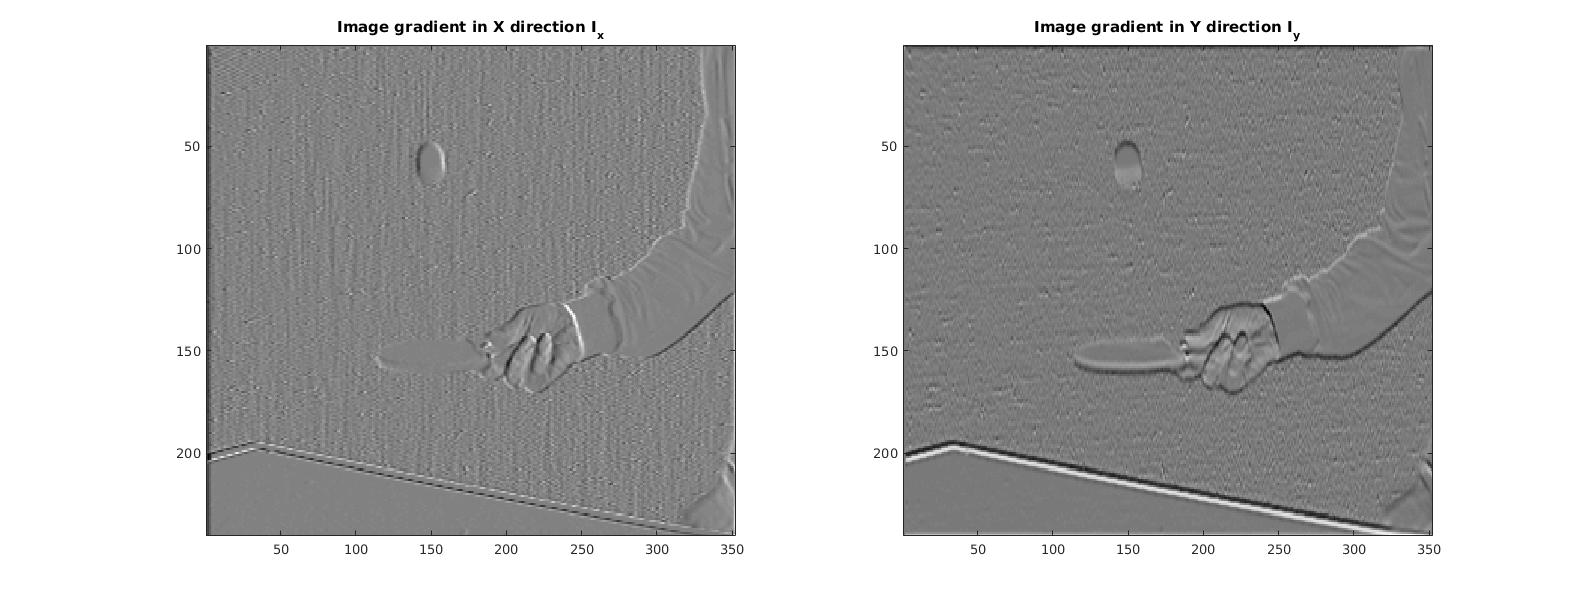
\includegraphics[width=1\textwidth]{imgs/derivatives_pingpong.jpg}
	\caption{Image gradients for first Ping Pong image}
	\label{fig:partialDerivatives_pingpong}
\end{figure}

\begin{figure}[H] \centering
	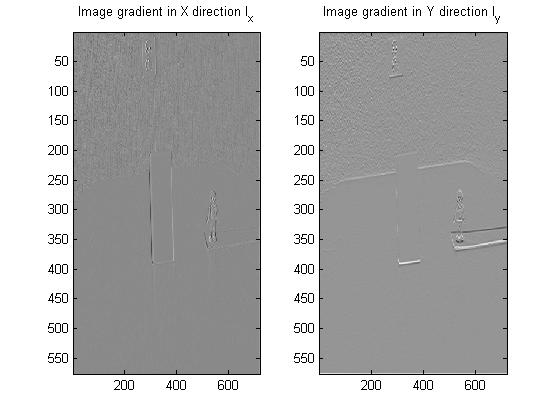
\includegraphics[width=1\textwidth]{imgs/derivatives_person.jpg}
	\caption{Image gradients for first Toy Person image}
	\label{fig:partialDerivatives_person}
\end{figure}

Then, we created the $Q$ matrix, first by squaring the gradients (i.e.
($I_x)^2$ and ($I_y)^2$) and multiplying them with each other (i.e. $I_x *
I_y$), and then by convolving the resulting with a Gaussian kernel. With these
components we were able to compute $H$ using Equation $12$ shown in the
assignment instructions. A visualization for the scaled surfaces are shown in
Figure \ref{fig:surface_pingpong} and \ref{fig:surface_person}.

\begin{figure}[H] \centering
	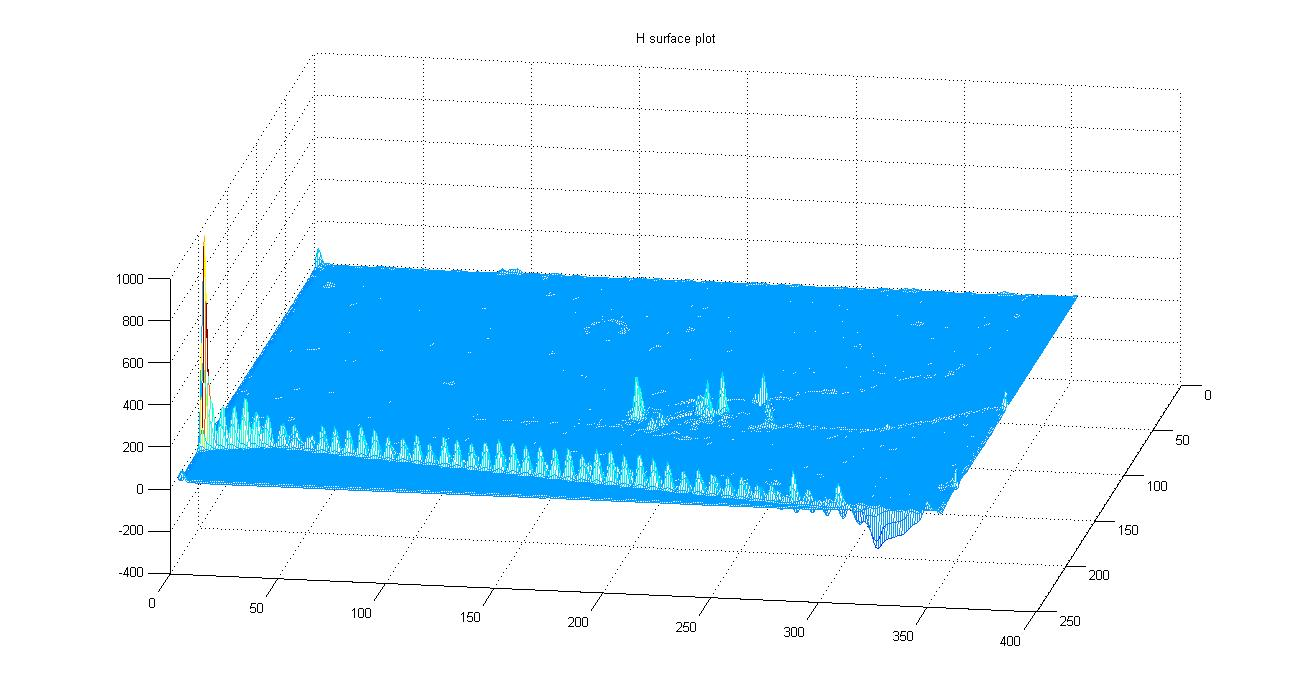
\includegraphics[width=1\textwidth]{imgs/surface_pingpong.jpg}
	\caption{$H$ surface for first Ping Pong image. Local maxima are
		observed along the ping pong table, and the hand.}
	\label{fig:surface_pingpong}
\end{figure}

\begin{figure}[H] \centering
	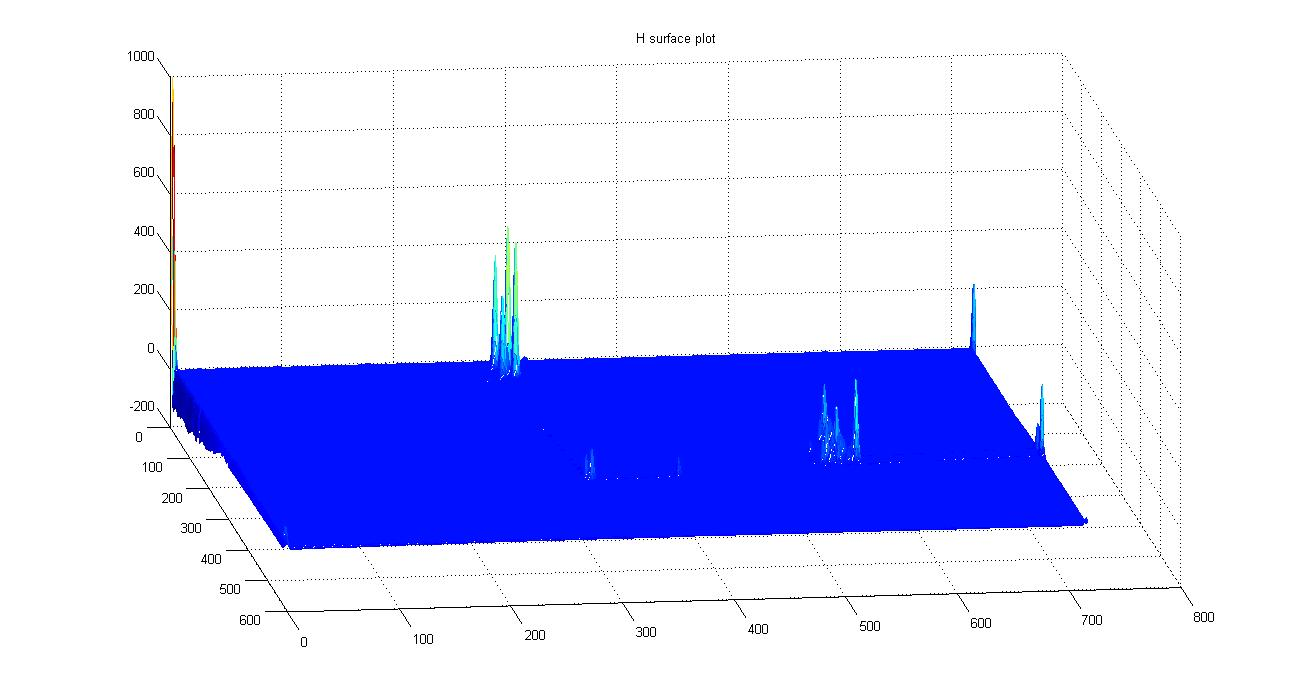
\includegraphics[width=1\textwidth]{imgs/surface_person.jpg}
	\caption{$H$ surface for first Toy Person image. Local maxima are
		observed on the power outlet and on the toy person.}
	\label{fig:surface_person}
\end{figure}

Finally, to choose the corner points we considered two conditions:
\begin{enumerate} 
	\item A corner point must be a local maximum. To check for
		this we need to compare its value with all its neighbors' within
		a given window.
	\item A corner point must have a higher $H$
		value than a given threshold.
\end{enumerate}

To create an accurate corner detector we need to tune the parameters. We noticed that smaller $\sigma$ had an effect of detecting more corner points on the background. A higher threshold results in more pressure to become a corner point and thus reduces the final number of points. Finally, a larger window size makes the corner points more sparse, and prevents the corner points to be clustered.

After tuning, the chosen values for the final detector are:
\begin{itemize}
	\item $kernel  length = 11$
	\item $\sigma = 1$
	\item $window  size = 3$
	\item $threshold = 7$
\end{itemize}

To validate our detector we compared it with the Matlab corner function. Quantitatively we get the number of corner points detected, so that our detector ideally has an output in the same order of magnitude as the Matlab detector. Additionally, we compared it qualitatively by visually plotting the corner points and checking both implementations detected about the same points.
 
\begin{figure}[H] \centering
	\begin{subfigure}{.5\textwidth} \centering
		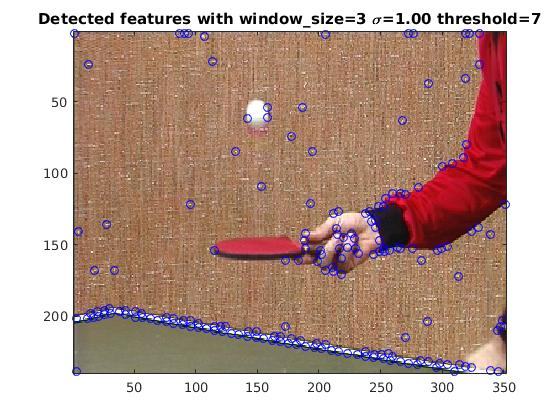
\includegraphics[width=.9\textwidth]{imgs/ourCorners_pingpong.jpg}
		\caption{Our implementation of Harris Corner Detector.}
		\label{fig:ourCorners_pingpong}
	\end{subfigure}%
	\begin{subfigure}{.5\textwidth}	\centering
		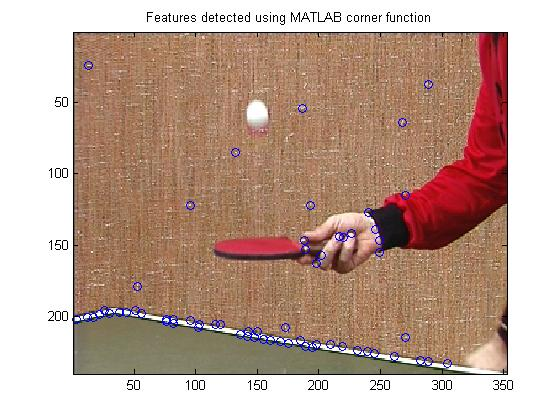
\includegraphics[width=.9\textwidth]{imgs/matlabCorners_pingpong.jpg}
		\caption{Matlab's built in Corner function.}
		\label{fig:matlabCorners_pingpong}
	\end{subfigure}
	\caption{Corner points in first Ping Pong image}
	\label{fig:corners_pingpong}
\end{figure}

\begin{figure}[H] \centering
	\begin{subfigure}{.5\textwidth} \centering
		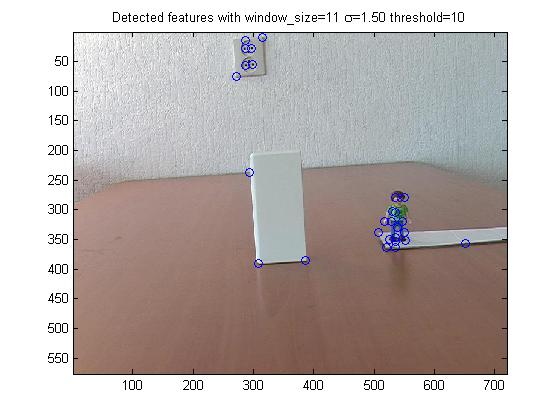
\includegraphics[width=.9\textwidth]{imgs/ourCorners_person.jpg}
		\caption{Our implementation of Harris Corner Detector.}
		\label{fig:ourCorners_person}
	\end{subfigure}%
	\begin{subfigure}{.5\textwidth}	\centering
		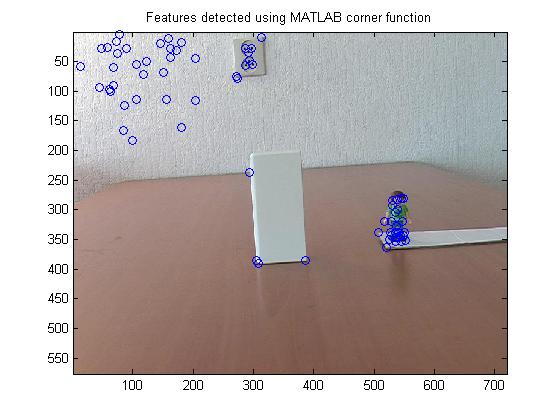
\includegraphics[width=.9\textwidth]{imgs/matlabCorners_person.jpg}
		\caption{Matlab's built in Corner function.}
		\label{fig:matlabCorners_person}
	\end{subfigure}
	\caption{Corner points in first Toy person image}
	\label{fig:corners_person}
\end{figure}

\section{Lucas-Kanade Algorithm for Optical Flow}


\section{Tracking}

\end{document}